% \setcounter{chapter}{1}
% \setcounter{section}{0}
\chapter{Построение вероятностной модели тандема}						% Заголовок
% \addcontentsline{toc}{chapter}{Построение вероятностной модели тандема}	% Добавляем его в оглавление


В разделе~1.1 вопрос об операции управления системой ставится на содержательном уровне. На первом этапе задача формулируется в терминах теории массового обслуживания: описываются входные потоки,   виды имеющихся очередей,  обслуживающее устройство и т.п. Особое внимание уделяется описанию графа переходов обслуживающего устройства,  имеющий нетривиальный характер. В качестве наглядной интерпретации системы приводится тандем перекрестков. 

Раздел~1.2 содержит построение строгой математической модели для управляющей системы,  которая была представлена в разделе~1.1. Данный этап является основополагающим для всего дальнейшего анализа. При построении модели существенно используется кибернетический подход и его основные принципы: наблюдение за системой совершается в дискретные моменты времени,   строятся функциональные и вероятностные соотношения между блоками функционирования системы,  а также описание блоков системы производится нелокально.
\section{Постановка задачи на содержательном уровне}
Рассмотрим систему массового обслуживания следующего вида (Рис.~\ref{SystemScheme}).
\begin{figure}[h]
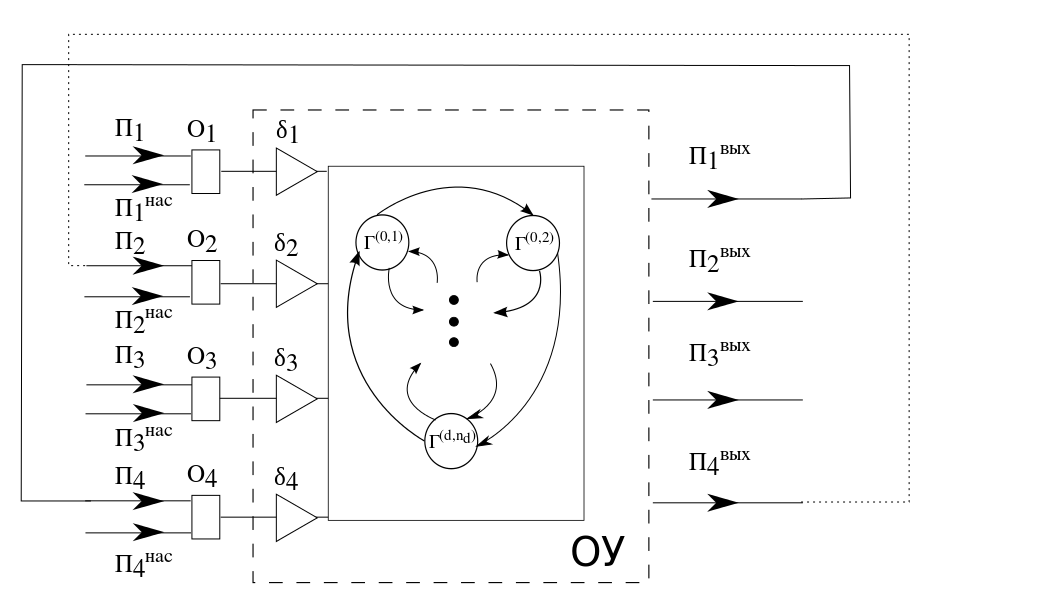
\includegraphics[scale=0.45]{Pictures/SystemScheme.png} 
\caption{Структурная схема системы обслуживания}
\label{SystemScheme}
\end{figure}
В систему,  осуществляющую операцию по обслуживанию одним обслуживающим устройством,  поступают потоки $\Pi_1$,  $\Pi_2$,  $\Pi_3$  и $\Pi_4$. Требования потока $\Pi_j$ приходят в соответствующую очередь $O_j$ неограниченного объема,  $j\in \{1,  2,  3,  4\}$. Дисциплина очереди $O_j$,  $j \in \{1,  2,  3\}$,  поддерживается при помощи устройства $\delta_j$ и имеет тип <<первым пришел~--- первым ушел>> (FIFO). Другими словами,  на обслуживание поступает требование,  пришедшее раньше остальных. Дисциплина очереди $O_4$ будет описана ниже. Будем предполагать,  что внешняя среда,  формирующая входные потоки $\Pi_1$ и $\Pi_3$,  имеет только одно состояние,  то есть вероятностная структура потоков не меняется с течением времени. 
Входящие потоки требований $\Pi_1$ и $\Pi_3$ являются неординарными пуассоновскими потоками,  то есть ординарными,  стационарными и без последействия потоками групп требований. Соответствующие простейшие потоки для $\Pi_1$ и $\Pi_3$ имеют интенсивности $\lambda_1$ и $\lambda_3$. При помощи следующей производящей функции зададим  распределение количества заявок в группе по потоку $\Pi_j$:
\begin{equation}
f_j(z) = \sum_{\nu=1}^{\infty} p_{\nu}^{(j)} z^{\nu},  \quad j\in \{1, 3\}.
\label{GeneratingFunc}
\end{equation}
Функцию $f_j(\cdot)$,  $j\in \{1, 3\}$,  будем предполагать аналитической при всех $z\in \mathbb{C}$ таких,  что $|z|\hm<(1+\varepsilon)$,  $\varepsilon>0$. Величина $p_{\nu}^{(j)}$ задает  вероятность того,  что по потоку $\Pi_j$ число требований в группе равно $\nu$. После обслуживания требования потока $\Pi_1$ повторно поступают в систему для обслуживания,  формируя при этом поток $\Pi_4$. Затем,  обслуженные требования потока $\Pi_4$ поступают на еще одно повторное обслуживание,  создавая при этом поток $\Pi_2$. Потоки $\Pi_2$ и $\Pi_3$ являются конфликтными,  что означает запрет на одновременное обслуживание требований этих потоков и,  следовательно,  исследование системы не может быть сведено к задаче с меньшим числом потоков. 

Обслуживающее устройство в каждый момент времени может находиться в одном из множества состояний $\Gamma=\{\Gamma^{(k, r)} \colon k=\overline{0, d}; r=\overline{1, n_k}\}$ с заданными натуральными числами $d$,  $n_0$,  $n_1$,  $\ldots$,  $n_d$. В каждом состоянии $\Gamma^{(k, r)}$ обслуживающее устройство находится в течение времени $T^{(k, r)}$. Введем множества $\Gamma^{\mathrm{I}}$,  $\Gamma^{\mathrm{II}}$, 
$\Gamma^{\mathrm{III}}$ и $\Gamma^{\mathrm{IV}}$ следующим образом. В состоянии $\gamma \in \Gamma^{\mathrm{I}}$ обслуживаются только требования из очередей $O_1$,  $O_2$ и $O_4$.
В состоянии $\gamma \in \Gamma^{\mathrm{II}}$ обслуживаются только требования из очередей $O_2$ и $O_4$.
В состоянии $\gamma \in \Gamma^{\mathrm{III}}$ обслуживаются только требования из очередей $O_1$,  $O_3$ и $O_4$.
В состоянии $\gamma \in \Gamma^{\mathrm{IV}}$ обслуживаются только требования из очередей $O_3$ и $O_4$.
Тогда множество $\Gamma$ есть объединение $\Gamma = \Gamma^{\mathrm{I}} \cup \Gamma^{\mathrm{II}} \cup \Gamma^{\mathrm{III}} \cup\Gamma^{\mathrm{IV}}$ непересекающихся подмножеств. Также в дальнейшем нам понадобятся множества ${}^1\Gamma=\Gamma^{\mathrm{I}} \cup \Gamma^{\mathrm{III}}$,  
${}^2\Gamma=\Gamma^{\mathrm{I}} \cup \Gamma^{\mathrm{II}}$, 
${}^3\Gamma=\Gamma^{\mathrm{III}} \cup \Gamma^{\mathrm{IV}}$. 

Смена состояний обслуживающего устройства осуществляется по следующему правилу. Множество состояний $C_k = \{\Gamma^{(k, r)} \colon r=\overline{1, n_k}\}$ будем называть $k$-м циклом,  $k=\overline{1, d}$ (Рис. \ref{GraphScheme}). Состояние вида $\Gamma^{(0, r)}$ будем называть состоянием продления,  $r=\overline{1, n_0}$. Положим $r \oplus_k 1 = r+1$ для $r=\overline{1, n_k-1}$ и $r \oplus_k 1 = 1$ при $r=n_k$,  $k = \overline{0, d}$. В цикле $C_k$ выделим подмножества $C_k^{\mathrm{O}}$ выходных,  $C_k^{\mathrm{I}}$ входных и $C_k^{\mathrm{N}} = C_k \setminus (C_k^{\mathrm{O}} \cup C_k^{\mathrm{I}})$ нейтральных состояний. Тогда после состояния $\Gamma^{(k, r)} \hm\in C_k\setminus C_k^{\mathrm{O}}$ обслуживающее устройство переходит в состояние $\Gamma^{(k, r \oplus_k 1)}$ того же цикла $C_k$. При $\Gamma^{(k, r)}$,  принадлежащем множеству $C_k^{\mathrm{O}}$,  прибор переходит в состояние $\Gamma^{(k, r \oplus_k 1)}$,  если число требований в очереди $O_3$ в момент переключения больше заданного порога $L$. В противном случае,  то есть если число требований в очереди $O_3$ меньше либо равно $L$,  новое состояние прибора будет состоянием продления $\Gamma^{(0, r_1)}$,  где $r_1=h_1(\Gamma^{(k, r)})$ и $h_1(\cdot)$~--- заданное отображение множества $\bigcup\limits_{k=1}^d C_k^{\mathrm{O}}$ во множество $\{1, 2, \ldots,  n_0\}$. После состояния $\Gamma^{(0, r)}$ выбирается состояние того же вида $\Gamma^{(0, r_2)}$,  если число требований в очереди $O_3$ меньше или равно $L$,  где $r_2=h_2(r)$ и $h_2(\cdot)$~--- заданное отображение множества $\{1, 2,  \ldots,  n_0\}$ на себя; в противном случае включается входное состояние $\Gamma^{(k, r_3)} \in C_k^{\mathrm{I}}$,  где $\Gamma^{(k, r_3)}=h_3(r)$ и $h_3(\cdot)$~--- заданное отображение множества $\{1, 2,  \ldots,  n_0\}$ на множество  $\bigcup\limits_{k=1}^d C_k^{\mathrm{I}}$. Считается,  что все состояния продления $\Gamma^{(0, r)}$ принадлежат множеству ${}^2 \Gamma$,  а также верны соотношения $C_k^\mathrm{O}\subset {}^2 \Gamma$ и $C_k^\mathrm{I}\subset {}^3 \Gamma$. Также будем предполагать,  что все циклы имеют ровно одно входное и одно выходное состояние. И последним предположением является то,  что все вершины продления образуют один цикл,  то есть можем положить $h_2(r)=r\oplus_0 1$.

\begin{figure}[h]\centering
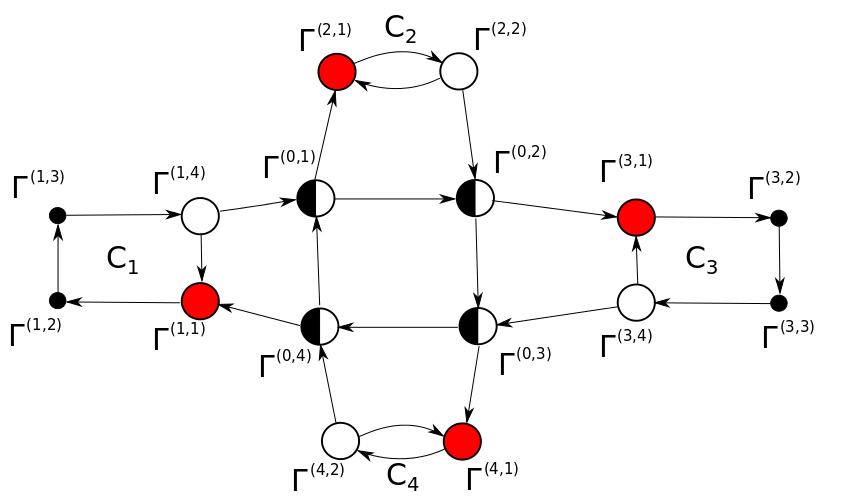
\includegraphics[scale=0.5]{Pictures/GraphScheme3.png} 
\caption{Класс графов переходов. Незакрашенные вершины являются выходными вершинами,  большие закрашенные вершины --- входные,  небольшие закрашенные --- нейтральные,  наполовину закрашенным вершинам соответствуют состояния продления}
\label{GraphScheme}
\end{figure}
%\subsection{Допустимые графы переходов состояний ОУ}

Таким образом,  смена состояний обслуживающего устройства задается соотношением:
\begin{equation}
h(\Gamma^{(k, r)}, y) = 
\begin{cases}
\Gamma^{(k, r \oplus_k 1)}, & \quad \text{если } (\Gamma^{(k, r)}\in C_k\setminus C_k^{\mathrm{O}}) \\
& \quad \text{или } (\Gamma^{(k, r)}\in C_k^{\mathrm{O}} \text{ и } y>L);\\
%\Gamma^{(k, r \oplus_k 1)}, & \quad \text{ если } \Gamma^{(k, r)}\in C_k^{\mathrm{O}} \text{ и } y>L;\\
\Gamma^{(0, h_1(\Gamma^{(k, r)}))}, & \quad \text{если } \Gamma^{(k, r)}\in C_k^{\mathrm{O}} \text{ и } y\leqslant L;\\
\Gamma^{(0, r \oplus_0 1)}, & \quad \text{если } k=0 \text{ и } y\leqslant L;\\
h_3(r), & \quad \text{если } k=0 \text{ и } y > L.
\end{cases}
\label{hLaw}
\end{equation}

Рассмотрим введеные обозначения на примере рис.~\ref{GraphScheme}. Входными состояниями обслуживающего устройства являются $\Gamma^{(1, 1)} \in C_1^{\mathrm{I}}$,  $\Gamma^{(2, 1)} \in C_2^{\mathrm{I}}$,  $\Gamma^{(3, 1)} \in C_3^{\mathrm{I}}$ и $\Gamma^{(4, 1)} \in C_4^{\mathrm{I}}$,  выходные состояния~--- $\Gamma^{(1, 4)} \in C_1^{\mathrm{O}}$,  $\Gamma^{(2, 2)} \in C_2^{\mathrm{O}}$,  $\Gamma^{(3, 4)} \in C_3^{\mathrm{O}}$ и $\Gamma^{(4, 2)} \in C_4^{\mathrm{O}}$,  нейтральные состояния~--- $\Gamma^{(1, 2)},  \Gamma^{(1, 3)} \in C_1^{\mathrm{N}}$ и $\Gamma^{(3, 2)},  \Gamma^{(3, 3)} \in C_3^{\mathrm{N}}$. Состояния продления на графе представлены вершинами $\Gamma^{(0, 1)}$,  $\Gamma^{(0, 2)}$,  $\Gamma^{(0, 3)}$ и $\Gamma^{(0, 4)}$. Далее,  отображение $h_1(\cdot)$ на графе задано таким образом,  что оно переводит,  например,  выходное состояние $\Gamma^{(1, 4)}$ в число $1$~--- номер состояния продления $\Gamma^{(0, 1)}$,  то есть $h_1(\Gamma^{(1, 4)})=1$. Аналогично,  например,  $h_2(1)=2$ и $h_2(3)=4$. Примером отображения $h_3(\cdot)$ является $h_3(2)=\Gamma^{(3, 1)}$.


Предполагается,  что длительности обслуживания различных требований могут  иметь различные законы распределения и,  вообще говоря,  быть зависимыми,  поэтому вместо привычного способа,  состоящего в указании функции распределения длительности обслуживания произвольного требования,  будут использованы потоки насыщения. Потоками насыщения $\Pi^{\mathrm{\text{нас}}}_j$,  $j=\overline{1, 4}$,  назовем виртуальные выходные потоки при условии максимального использования ресурсов обслуживающего устройства,  а для $j=\overline{1, 3}$ еще и при условии максимальной загрузки соответствующих очередей.
Более конкретно,  поток насыщения $\Pi^{\mathrm{\text{нас}}}_j$,  $j=\overline{1, 3}$,  содержит неслучайное число $\ell(k, r, j)$ требований,  которые были обслужены в течение времени $T^{(k, r)}$,  если обслуживающее устройство находилось в состоянии $\Gamma^{(k, r)}$. Пусть $\mathbb{Z}_+$~--- множество целых неотрицательных чисел. Тогда,  при условии,  что в очереди $O_4$ находится $x \in \mathbb{Z}_+$ требований,  поток насыщения $\Pi^{\mathrm{\text{нас}}}_4$ определим как поток,  содержащий все $x$ требований.
%\subsection{Пример: тандем из двух перекрестков} 
Наконец,  при состоянии обслуживающего устройства $\Gamma^{(k, r)}$ каждое требование из очереди $O_4$ с вероятностью $p_{k, r}$ и независимо от других завершает обслуживание и отправляется в очередь $O_2$ потока~$\Pi_2$. С вероятностью $1-p_{k, r}$ требование очереди $O_4$ остается в ней до следующего такта. На следующем такте процесс повторяется.

В качестве наглядной физической интерпретации можно привести тандем из двух перекрестков (рис. \ref{crossroads}).
\begin{figure}[h]\centering
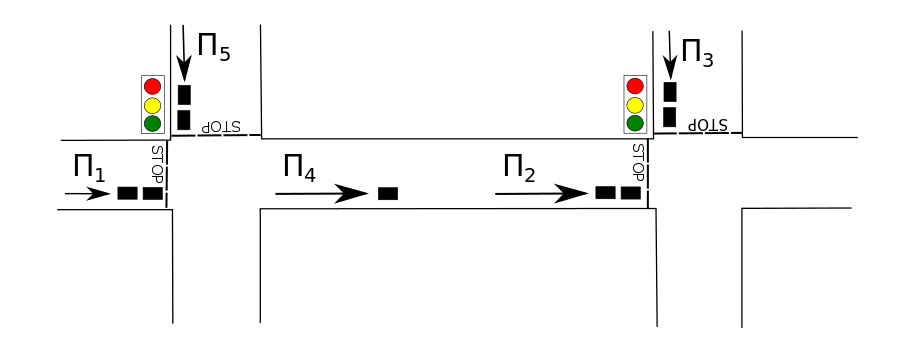
\includegraphics[scale=0.5]{Pictures/Crossroads.png} 
\caption{Пример: тандем перекрестков}
\label{crossroads}
\end{figure}
В качестве потоков требований,  формируемых внешней средой,  выступают потоки прибывающих на перекрестки машин: конфликтные потоки $\Pi_1$,  $\Pi_5$ на первом перекрестке,  а также поток $\Pi_3$ на втором. Каждая машина из потока $\Pi_1$,  проезжая первый перекресток,  становится в очередь $O_4$ потока $\Pi_4$ и затем с некой вероятностью ($p_{k, r}$ для состояния $\Gamma^{(k, r)}$ обслуживающего устройства) доезжает до следующего перекрестка,  или же не успевает это сделать и остается в очереди $O_4$ до следующего такта обслуживания. В случае,  если машина из очереди $O_4$ успевает доехать до второго перекрестка,  она становится в очередь $O_2$ и ждет своей очереди для его прохождения.

Предполагается,  что светофор на первом перекрестке имеет лишь два состояния $\{g_{1, 1}, g_{1, 2}\}$: в состоянии $g_{1, 1}$ машины потока $\Pi_1$ пропускаются фиксированное количество времени $\widetilde T^{(1, 1)}$ (<<зеленый>> свет для $\Pi_1$); в состоянии $g_{1, 2}$ --- простаивают в течение времени $\widetilde T^{(1, 2)}$ (<<красный>> свет для $\Pi_1$). Светофор на втором перекрестке обслуживает по алгоритму с продлением: дополнительно к состоянию обслуживания потока $\Pi_3$ (состояние $g_{2, 1}$),  также имеется два состояния обслуживания потока $\Pi_2$ (состояния $g_{2, 2}$,  $g_{2, 3}$). Первое из них включается всегда после завершения обслуживания потока $\Pi_3$,  а второе включается,  если после очередного такта обслуживания потока $\Pi_2$ длина очереди $O_3$ не превосходит уровня $L$.
Длительности пребывания светофора на втором перекрестке в каждом из состояний суть $\widetilde T^{(2, 1)}$,  $\widetilde T^{(2, 2)}$ и $\widetilde T^{(2, 3)}$.


Рассматривая тандем из двух перекрестков как единую систему массового обслуживания и предполагая наблюдение за ней только в (дискретные) моменты переключения состояния хотя бы одного из светофоров,  может быть показано,  что количество различных состояний у полученной системы конечно. Действительно,  положим,  например,  за состояние объединенной системы вектор $(g^{(1)},  g^{(2)},  s,  t)$,  где $g^{(1)}\in \{g_{1,  1},  g_{1,  2}\}$~--- состояние $1$--го перекрестка,  $g^{(2)}\in \{g_{2,  1},  g_{2,  2},  g_{2,  3}\}$~--- состояние $2$--го перекрестка,  $s \in \{0,  1,  2\}$~--- номер последнего сменившего состояние перекрестка (принимает значение $0$ в случае,  если сменили состояние оба перекрестка) и $t \in \{0,  1,  2,  \ldots,  T\}$~--- количество времени,  оставшееся у продолжающего обслуживание с прошлого такта перекрестка (принимает значение $0$,  если принимает значение $0$ величина $s$). Здесь $T$~--- максимальная длительность нахождения каждого из светофоров в одном состоянии. Тогда количество различных состояний не трудно посчитать и оно не будет превышать величины  $2\times 3 \times 3 \times T$.

В завершении построения примера отметим,  что при прохождении перекрестков машины предполагаются движущимися только в прямом направлении,  то есть перемешивания конфликтных потоков не допускается. Таким образом,  поток $\Pi_5$ не представляет интереса для дальнейшего исследования системы и может быть отброшен и,  следовательно,  построенный пример целиком удовлетворяет структурной схеме на рис.~\ref{SystemScheme}.

Теперь продемонстрируем на конкретном числовом примере выделение циклов и состояний продления. Пусть изменение состояний перекрестков и время пребывания (в секундах,  для определенности) в каждом из состояний задается графами на рис. \ref{SystemStates}.
\begin{figure}[h]\centering
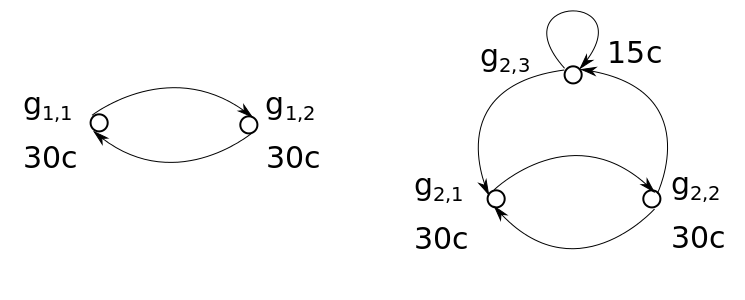
\includegraphics[scale=0.5]{Pictures/SystemStates.png} 
\caption{Числовой пример тандема перекрестков. Левый граф соответствует первому перекрестку,  правый~--- второму}
\label{SystemStates}
\end{figure}
За начальное состояние объединенной системы примем $\Gamma_0=(g_{1,  1},  g_{2,  1},  0,  0)$,  то есть первый перекресток находится в состоянии $g_{1, 1}$,  второй~--- в состоянии $g_{2,  1}$,  и оба только начали свою работу в своем состоянии (этот факт моделируется равенствами $s=0$ и $t=0$). Следующая смена состояний случится у обоих перекрестков одновременно и приведет к следующему состоянию $(g_{1,  2},  g_{2,  2},  0,  0)$. Далее смена состояний произойдет также у первого и второго перекрестков,  однако второй перекресток может перейти как в состояние $g_{2,  1}$,  так и в состояние продления $g_{2,  3}$. Таким образом,  следущим состоянием тандема будет либо опять $(g_{1,  1},  g_{2,  1},  0,  0)$,  либо $(g_{1,  1},  g_{2,  3},  0,  0)$. Продолжая рассуждения аналогичным образом,  получим следущий список всех возможных состояний системы:
\begin{align*}
(g_{1,  1},  g_{2,  1},  0,  0)&=\Gamma^{(1,  1)} ,  & \quad (g_{1,  2},  g_{2,  2},  0,  0)&=\Gamma^{(1,  2)} ,  & \quad (g_{1,  1},  g_{2,  3},  0,  0)&=\Gamma^{(0,  1)},   \\
(g_{1,  1},  g_{2,  3},  15,  2)&=\Gamma^{(0,  2)} ,  & \quad (g_{1,  2},  g_{2,  3},  0,  0)&=\Gamma^{(0,  3)} ,  & \quad (g_{1,  2},  g_{2,  3},  15,  2)&=\Gamma^{(0,  4)},   \\
(g_{1,  2},  g_{2,  1},  15,  2)&=\Gamma^{(4,  1)} ,  & \quad (g_{1,  1},  g_{2,  1},  15,  1)&=\Gamma^{(4,  2)} ,  & \quad (g_{1,  1},  g_{2,  2},  15,  2)&=\Gamma^{(4,  3)},   \\
(g_{1,  2},  g_{2,  2},  15,  1)&=\Gamma^{(4,  4)} ,  & \quad (g_{1,  2},  g_{2,  3},  15,  2)&=\Gamma^{(0,  5)} ,  & \quad (g_{1,  2},  g_{2,  1},  0,  0)&=\Gamma^{(3,  1)},   \\
(g_{1,  1},  g_{2,  2},  0,  0)&=\Gamma^{(3,  2)} ,  & \quad (g_{1,   1},  g_{2,  1},  15,  2)&=\Gamma^{(2,  1)} ,  & \quad (g_{1,  2},  g_{2,  1},  15,  1)&=\Gamma^{(2,  2)},   \\
(g_{1,  2},  g_{2,  2},  15,  2)&=\Gamma^{(2,  3)} ,  & \quad (g_{1,  1},  g_{2,  2},  15,  1)&=\Gamma^{(2,  4)}. & &
\end{align*}
В соответствии с приведенными выше обозначениями,   множества $C_1$,  $C_2$,  $C_3$,  $C_4$,  а также множество состояний продления строятся однозначным образом. Множествами входных состояний будут $C_1^{\mathrm{I}}=\{\Gamma^{(1,  1)}\}$,  $C_2^{\mathrm{I}}=\{\Gamma^{(2,  1)}\}$,  $C_3^{\mathrm{I}}=\{\Gamma^{(3,  1)}\}$ и $C_4^{\mathrm{I}}=\{\Gamma^{(4,  1)}\}$. Множествами выходных состояний будут $C_1^{\mathrm{O}}=\{\Gamma^{(1,  2)}\}$,  $C_2^{\mathrm{O}}=\{\Gamma^{(2,  4)}\}$,  $C_3^{\mathrm{O}}=\{\Gamma^{(3,  2)}\}$ и $C_4^{\mathrm{O}}=\{\Gamma^{(4,  4)}\}$. Функции $h_1(\cdot)$,  $h_2(\cdot)$ и $h_3(\cdot)$ задаются поточечно:
\begin{equation*}
h_1(\Gamma^{(1,  2)})=1,  \quad h_1(\Gamma^{(2,  4)})=2,  \quad h_1(\Gamma^{(3,   2)})=3,  \quad h_1(\Gamma^{(4,  4)})=5, 
\end{equation*}
\begin{equation*}
h_2(1)=2,  \quad h_2(2)=3,  \quad h_2(3)=4 \quad h_2(4)=1,  \quad h_2(5)=1, 
\end{equation*}
\begin{equation*}
h_3(1)=\Gamma^{(2, 1)},  \quad h_3(2)=\Gamma^{(3, 1)},  \quad h_3(3)=\Gamma^{(4, 1)} \quad h_3(4)=\Gamma^{(1, 1)},  \quad h_3(5)=\Gamma^{(1, 1)}.
\end{equation*}
Этим завершается построение числового примера.

\section{Представление рассматриваемой системы обслуживания в виде кибернетической управляющей системы}
Описанная в предыдущем разделе на содержательном уровне система массового обслуживания должна рассматриваться как кибернетическая управляющая система обслуживания (см. \cite{Zorin:2011:2}). Схема управляющей системы представлена на рис. \ref{SystemScheme}. Схема состоит из следующих блоков: 1)~входные полюса первого типа~--- входные потоки $\Pi_1$,  $\Pi_2$,  $\Pi_3$,  $\Pi_4$; 2)~входные полюса второго типа~--- потоки насыщения $\Pi_1^{\mathrm{\text{нас}}}$,  $\Pi_2^{\mathrm{\text{нас}}}$,  $\Pi_3^{\mathrm{\text{нас}}}$,  $\Pi_4^{\mathrm{\text{нас}}}$; 3)~выходные полюса $\Pi_1^{\mathrm{\text{вых}}}$,  $\Pi_2^{\mathrm{\text{вых}}}$,  $\Pi_3^{\mathrm{\text{вых}}}$,  $\Pi_4^{\mathrm{\text{вых}}}$; 4)~внутренняя память~--- обслуживающее устройство (ОУ);  5)~устройство по переработке информации внутренней памяти~--- граф смены состояний;  6)~внешняя память~--- очереди $O_1$,  $O_2$,  $O_3$,  $O_4$; 7)~устройство по переработкe информации внешней памяти~--- устройства по поддержанию дисциплины очереди $\delta_1$,  $\delta_2$,  $\delta_3$,  $\delta_4$; 8) внешняя среда с одним состоянием. Координатой блока является номер этого блока на схеме.

Зададим информацию о блоках с помощью следующих случайных величин и элементов,  указав,  в том числе,  множества их возможных значений. В качестве дискретной временной шкалы выберем последовательность $\tau_0=0$,  $\tau_1$,  $\tau_2$,  $\ldots$ моментов смены состояния обслуживающего устройства. Обозначим:
\begin{itemize}
\item $\Gamma_i$,  $i\geqslant 1$,  из множества $\Gamma$~--- состояние обслуживающего устройства в течение времени $\left(\tau_{i-1};\tau_i\right]$ и $\Gamma_0\in \Gamma$~--- в момент времени $\tau_0$;
\item количество $\varkappa_{j, i} \in \mathbb{Z}_+ $,  $i\geqslant 0$,  требований в очереди $O_j$ в момент времени $\tau_i$;
\item количество $\eta_{j, i} \in \mathbb{Z}_+$,  $i\geqslant 0$,  требований,  поступивших в очередь $O_j$ по потоку $\Pi_j$ в течение времени $\left(\tau_{i};\tau_{i+1}\right]$;
\item количество $\xi_{j, i} \in \mathbb{Z}_+$,  $i\geqslant 0$,  требований по потоку насыщения $\Pi^{\mathrm{\text{нас}}}_j$ в течение времени $\left(\tau_{i};\tau_{i+1}\right]$;
\item количество $\overline{\xi}_{j, i}\in \mathbb{Z}_+$,  $i\geqslant 0$,  реально обслуженных требований по потоку $\Pi_j$ в течение времени $\left(\tau_{i};\tau_{i+1}\right]$; $j=\overline{1, 4}$.
\end{itemize}
Закон изменения состояния обслуживающего устройства будем предполагать заданным соотношением 
\begin{equation}
\Gamma_{i+1}=h(\Gamma_i,  \varkappa_{3, i}), 
\label{gammaFunc}
\end{equation}
где отображение $h(\cdot,  \cdot)$ определено в \eqref{hLaw}.
Для определения длительности $T_{i+1}$ состояния обслуживающего устройства в течение времени $\left(\tau_{i};\tau_{i+1}\right]$ удобно ввести функцию $h_T(\cdot,  \cdot)$:
\begin{equation*}
T_{i+1}=h_T(\Gamma_i,  \varkappa_{3,  i})= T^{(k,  r)}, \quad  \text{ где $k$ и $r$ таковы,  что } \Gamma^{(k,  r)}=\Gamma_{i+1}=h(\Gamma_i, \varkappa_{3,  i}).
%\label{timeLaw}
\end{equation*}
Функциональная зависимость
\begin{equation}
\overline{\xi}_{j,  i}=\min\{\varkappa_{j,  i}+\eta_{j,  i},  \xi_{j,  i}\},  \quad j \in \{1,  2,  3\}, 
\label{saturationEq}
\end{equation}
между величиной $\overline{\xi}_{j, i}$ и величинами $\varkappa_{j, i}$,  $\eta_{j, i}$,  $\xi_{j, i}$ реализует стратегию механизма обслуживания требований. Далее,  поскольку 
\begin{equation*}
\varkappa_{j,  i+1}=\varkappa_{j,  i}+\eta_{j,  i}-\overline{\xi}_{j,  i},  \quad  j \in \{1,  2,  3\}, 
\end{equation*}
то из выражения \eqref{saturationEq} следует соотношение
\begin{equation}
\varkappa_{j,  i+1}=\max\{{0,  \varkappa_{j,  i}+\eta_{j,  i}-\xi_{j,  i}}\},  \quad j \in \{1,  2,  3\}.
\label{queuesFunc}
\end{equation}
Из формулировки поставленной задачи (см. также структурную схему на рис.~\ref{SystemScheme}) следуют соотношения для потока $\Pi_4$:
\begin{equation}
\eta_{4, i} = \min\{\xi_{1, i},  \varkappa_{1, i}+\eta_{1, i}\},  \quad \varkappa_{4, i+1}=\varkappa_{4, i}+\eta_{4, i}-\eta_{2, i},  \quad \xi_{4, i} = \varkappa_{4, i}.
\label{FourthFunc}
\end{equation}

Нелокальное описание входных потоков и потоков насыщения состоит в указании некоторых свойств условных распределений выделенных дискретных компонент $\eta_i=(\eta_{1,  i},  \eta_{2,  i},  \eta_{3,  i},  \eta_{4,  i})$ и $\xi_i \hm{=} (\xi_{1,  i},  \xi_{2,  i},  \xi_{3,  i},  \xi_{4,  i})$ маркированных точечных процессов  $\{(\tau_i,  \nu_i,  \eta_i); i\geqslant 0\}$ и $\{(\tau_i,  \nu_i,  \xi_i); i\geqslant 0\}$ при фиксированных значениях метки $\nu_i \hm= (\Gamma_i; \varkappa_i)$,  где $\varkappa_i=(\varkappa_{1,  i},  \varkappa_{2,  i},  \varkappa_{3,  i},  \varkappa_{4,  i})$. 
Введем функции $\varphi_1(\cdot,  \cdot)$ и $\varphi_3(\cdot,  \cdot)$ из разложений 
\begin{equation*}
\sum_{\nu=0}^{\infty} z^\nu\varphi_j(\nu,  t) = \exp\{\lambda_j t (f_j(z)-1)\}, 
\end{equation*}
где $f_j(z)$ определены выражением \eqref{GeneratingFunc},  $j \in \{1, 3\}$. Функция $\varphi_j(\nu,  t)$ по своему смыслу есть вероятность поступления $\nu=0$,  $1$,  $\ldots$ требований по потоку $\Pi_j$ за промежуток времени от $0$ до $t \geqslant 0$. Положим $\varphi_j(\nu, t)$ равной нулю при $\nu < 0$. Функцию $\psi(\cdot,  \cdot,  \cdot)$ зададим формулой
\begin{equation*}
\psi(k;y, u)=C_y^k u^k (1-u)^{y-k}.	
\end{equation*}
По своему смыслу $\psi(k; y,  u)$ есть вероятность поступления $k$ требований по потоку $\Pi_2$ при условии,  что очередь $O_4$ содержит $y$ требований и обслуживающее устройство находится в состоянии $\Gamma^{(k,  r)}$,  так что $u=p_{k,  r}$. При нарушении условия $ 0\leqslant k \leqslant y$ положим $\psi(k; y,  u)$ равной нулю.

Пусть $a=(a_1,  a_2,  a_3,  a_4) \in \mathbb{Z}_+^4$ и $x=(x_1,  x_2,  x_3,  x_4) \in \mathbb{Z}_+^4$. Тогда из постановки задачи на содержательном уровне следует,  что при фиксированном значении метки $\nu_i=(\Gamma^{(k,  r)}; x)$ вероятность $\varphi(a,  k,  r,  x)$ одновременного выполнения равенств $\eta_{1,  i}=a_1$,  $\eta_{2,  i}=a_2$,  $\eta_{3,  i}=a_3$,  $\eta_{4,  i}=a_4$ есть 
\begin{equation}
\varphi_1(a_1,  h_T(\Gamma^{(k,  r)},  x_3)) \times \psi(a_2,  x_4,  p_{\tilde{k},  \tilde{r}}) \times \varphi_3(a_3,  h_T(\Gamma^{(k,  r)},  x_3))
\times \delta_{a_4,  \min{\{\ell(\tilde{k},  \tilde{r},  1),  x_1+a_1}\}}, 
\label{conditionProbOne}
\end{equation}
где $\tilde{k}$ и $\tilde{r}$ таковы,  что $\Gamma^{(\tilde{k},  \tilde{r})}=h(\Gamma^{(k,  r)},  x_3)$ и $\delta_{i,  j}$ есть символ Кронекера:
%\begin{equation*}
$$
\delta_{i,  j}=
\begin{cases} 
1, & \quad \text{ если $i=j$, }\\
0, & \quad \text{ если $i\neq j$.}
\end{cases}
$$%\end{equation*}
Пусть $b=(b_1,  b_2,  b_3,  b_4) \in \mathbb{Z}_+^4$. Из содержательной постановки задачи также следует,  что вероятность $\zeta(b,  k,  r,  x)$ одновременного выполнения равенств $\xi_{1,  i}\hm=b_1$,  $\xi_{2,  i}=b_2$,  $\xi_{3,  i}=b_3$,  $\xi_{4,  i}=b_4$ при фиксированном значении $(\Gamma^{(k,  r)}; x)$ метки $\nu_i$ есть
\begin{equation}
\delta_{b_1,  \ell(\tilde{k},  \tilde{r},  1)} \times \delta_{b_2,  \ell(\tilde{k},  \tilde{r},  2)} \times 
\delta_{b_3,  \ell(\tilde{k},  \tilde{r},  3)} \times \delta_{b_4,  x_4}.
\label{conditionProbTwo}
\end{equation}
Из формулы \eqref{conditionProbTwo} следует для $j\in \{1,  2,  3\}$,  что вероятность события $\xi_{j,  i}=0$ равна $1$ в случае $h(\Gamma^{(k,  r)},  x_3)\notin {}^j\Gamma$ и что вероятность события $\xi_{j, i}=\ell(\tilde{k},  \tilde{r},  j)$ равна $1$,  если $\Gamma^{(\tilde{k},  \tilde{r})}=h(\Gamma^{(k,  r)},  x_3)\in {}^j\Gamma$.


Содержательный смысл следующей теоремы состоит в том,  что сформулированные выше функциональные связи и вероятностные свойства введенных объектов непротиворечивы и могут быть реализованы на некотором вероятностном пространстве.
%Построим теперь 	вероятностное пространство $(\Omega,  {\mathcal F},  \Pr(\cdot))$,  чтобы можно было рассматривать введеные величины как случайные величины на этом пространстве. А именно,  докажем следующую теорему.

\begin{theorem}
Пусть $\gamma_0=\Gamma^{(k_0,  r_0)}\in \Gamma$ и $x^0=(x_{1,  0},  x_{2,  0},   x_{3,  0},  x_{4,  0})\in \mathbb{Z}_+^4$ фиксированы.
Тогда существует вероятностное пространство $(\Omega,   {\mathcal F},   \Pr(\cdot))$ и заданные на нем случайные величины $\eta_{j,  i}=\eta_{j,  i}(\omega)$,   $\xi_{j,  i}=\xi_{j,  i}(\omega)$,   	 $\varkappa_{j,  i}=\varkappa_{j,  i}(\omega)$ и случайные элементы $\Gamma_i=\Gamma_i(\omega)$,   $i\geqslant 0$,   $j\in \overline{1,  4}$,   такие,   что 1) имеют место равенства $\Gamma_0(\omega) = \gamma_0$ и $\varkappa_0(\omega)=x^0$; 2) выполняются соотношения \eqref{gammaFunc},   \eqref{queuesFunc},   \eqref{FourthFunc}; 3) для любых  $a\in \mathbb{Z}_+^4$,   $b\in \mathbb{Z}_+^4$ и любых $x^t=(x_{1,  t},  x_{2,  t},  x_{3,  t},  x_{4,  t}) \in \mathbb{Z}_+^4$,   $\Gamma^{(k_t,  r_t)} \in \Gamma$,   $t = 1,   2,   \ldots$,   таких,   что $\Pr\Bigl(\bigcap\limits_{t=0}^{i}\{\omega\colon \Gamma_t=\Gamma^{(k_t,  r_t)},   \varkappa_t=x^t\}\Bigr)>0$,   условное распределение векторов $\eta_i$ и $\xi_i$,   $i \geqslant 0$,    имеет вид
\begin{multline}
\Pr \Bigl(\{ \omega \colon \eta_i = a,   \xi_i=b\} \,\,\Big
|\bigcap_{t=0}^{i}\{\omega\colon \Gamma_t=\Gamma^{(k_t,  r_t)},   \varkappa_t=x^t\}\Bigr)= \\=
\varphi(a,  k_i,  r_i,  x^i)\times \zeta(b,  k_i,  r_i,  x^i),  
\label{ProbablititiesToProve}
\end{multline}
где функции $\varphi(\cdot,   \cdot,   \cdot,   \cdot)$ и $\zeta(\cdot,   \cdot,   \cdot,   \cdot)$ определяются формулами \eqref{conditionProbOne} и \eqref{conditionProbTwo}.

\label{myTheorem}
\end{theorem}
\begin{proof}
Для построения вероятностного пространства $(\Omega,   {\mathcal F},   \Pr(\cdot))$ воспользуемся теоремой Ионеску Тулча (см. \cite{Shiryaev},   c. 348). 

Введем последовательность измеримых пространств $(\Omega_0,   {\mathcal F}_0)$,   $(\Omega_1,   {\mathcal F}_1)$,   $\ldots$,   где $\Omega_i\hm=\mathbb{Z}_+^3$,   $\omega_i=(\omega_{1,  i},  \omega_{2,  i},  \omega_{3,  i}) \hm\in \Omega_i$,   а $\sigma$-алгебра ${\mathcal F}_i=2^{\Omega_i}$  есть множество всех подмножеств множества $\Omega_i$. 
Пусть $\Gamma^{(\tilde{k},  \tilde{r})}=h(\Gamma^{(k_0,  r_0)},  x_{3,  0})$.
Зададим на измеримом пространстве $(\Omega_0,   {\mathcal F}_0)$ вероятностную меру $P_0(\cdot)$ ее значениями на одноточечных множествах:
\begin{multline}
P_0(\{(a_1,  a_2,  a_3)\})=\\=\varphi_1(a_1,  h_T(\Gamma^{(k_0,  r_0)})) \times \psi(a_2,  x_{2,  0},   p_{\tilde{k},  \tilde{r}}) \times \varphi_3(a_3,  h_T(\Gamma^{(k_0,  r_0)})).
\label{probabilitiesOne}
\end{multline}

Для $j\in \{1,  2,  3\}$ определим величины
\begin{equation}
\tilde{\Gamma}_0(\omega_0)=\gamma_0,  \quad \tilde{\varkappa}_{j,  0}(\omega_0)=x_{j,  0},   \quad \tilde{\xi}_{j,  0}(\omega_0)=l(\tilde{k},  \tilde{r},  j),   \quad \tilde{\eta}_{j,  0}(\omega_0)=\omega_{j,  0},  
\label{startRekOne}
\end{equation}
и
\begin{equation}
\begin{aligned}
 &\tilde{\varkappa}_{4,  0}(\omega_0)=x_{4,  0},   \quad \tilde{\xi}_{4,  0}(\omega_0)=x_{4,  0},  \\
&\tilde{\eta}_{4,  0}(\omega_0)=\min\{\tilde{\xi}_{1,  0}(\omega_0),   \tilde{\varkappa}_{1,  0}(\omega_0)+\tilde{\eta}_{1,  0}(\omega_0)\}
\end{aligned}
\label{startRekTwo}
\end{equation}

Теперь предположим,   что заданы вероятностные меры $$
P_i(\omega_0\hm{},  \omega_1, \hm{} \ldots \hm{},  \omega_{i-1};\cdot)
$$
на измеримых пространствах $(\Omega_i,  {\mathcal F}_i)$,  $i=\overline{0,  n}$,  
и 
% определеныслучайные величины $\tilde{\Gamma}_i$,  $\tilde{\varkappa}_{j, i}$,  $\tilde{\xi}_{j, i}$,  $\tilde{\eta}_{j, i}$,  ч,  и 
фиксирован набор $(\omega_0,  \omega_1,  \hm\ldots,  \omega_{n})$. Положим для $j\in \{1,  2,  3\}$  и $i=\overline{0,  n}$
\begin{equation}
\tilde{\Gamma}_{i+1}=\Gamma^{(k^*,  r^*)}=h(\tilde{\Gamma}_{i},  \tilde{\varkappa}_{3,  i}),   \quad \tilde{\varkappa}_{j,  i+1}=\max\{ 0,  \tilde{\varkappa}_{j,  i}+\tilde{\eta}_{j,  i} -\tilde{\xi}_{j,  i}\},  
\label{NextRekOne}
\end{equation}
\begin{equation}
\tilde{\varkappa}_{4,  i+1}=\tilde{\varkappa}_{4,  i}+\tilde{\eta}_{4,  i}-\tilde{\eta}_{2,  i},   \quad \tilde{\xi}_{j,  i+1}=l(k^*,  r^*,  j),  \quad \tilde{\eta}_{j,  i+1}=\omega_{j,  i+1},
\label{NextRekTwo}
\end{equation}
\begin{equation}
\tilde{\eta}_{4,  i+1}=\min\{\tilde{\xi}_{1,  i+1},   \tilde{\varkappa}_{1,  i+1}+\tilde{\eta}_{1,  i+1}\},   \quad \tilde{\xi}_{4,  i+1}=\tilde{\varkappa}_{4,  i+1}.
\label{NextRekThree}
\end{equation}
Заметим,   что значения $\tilde{\Gamma}_{i}$,   $\tilde\xi_{j,  i}$,   $\tilde\eta_{j,  i}$,   $\tilde\varkappa_{j,  i}$,   найденные по формулам \eqref{NextRekOne}--\eqref{NextRekThree} по наборам $(\omega_0,   \omega_1,  \ldots,   \omega_n)$ и $(\omega_0,   \omega_1,  \ldots,   \omega_i)$,   $n\geqslant i$,   совпадают.
Определим на измеримом пространстве $(\Omega_{n+1},   {\mathcal F}_{n+1})$ вероятностную меру  $P_{n+1}(\omega_0,   \omega_1,   \hm\ldots,   \omega_n;\cdot)$
ее значениями на одноточечных множествах $\{(a_1,  a_2,  a_3)\}$,   $(a_1,  a_2,  a_3)\hm\in {\mathbb Z}_+^3$:
\begin{multline}
P(\omega_0,  \omega_1,  \ldots,  \omega_n;\{(a_1,  a_2,  a_3)\}) = \\
= \varphi_1(a_1,  h_T(\tilde{\Gamma}_n,  \tilde{\varkappa}_{3,  n})) \times \psi(a_2,  \tilde{\varkappa}_{4,  n},   p_{k^*,  r^*}) \times \varphi_3(a_3,  h_T(\tilde{\Gamma}_n,  \tilde{\varkappa}_{3,  n})).
\label{probabilitiesTwo}
\end{multline}

%причем для любого множества $B\in {\mathcal F}_i$ функции $P(\omega_0, \omega_1, \hm\ldots,   \omega_{i-1};B)$ должны быть измеримыми функциями от $(\omega_0,  \omega_1,  \ldots,  \omega_{i-1})$. 


Тогда (в соответствии с теоремой Ионеску Тулчи) для декартова произведения $\Omega=\prod\limits_{i=0}^{\infty}\Omega_i$ пространств элементарных исходов и произведения $\sigma$-алгебр ${\mathcal F}=\bigotimes\limits_{i=0}^{\infty} {\mathcal F}_i$ на $(\Omega,  {\mathcal F})$ будет существовать единственная вероятностная мера $\Pr(\cdot)$ такая,   что для любого $i \geqslant 0$ верно равенство
\begin{equation}
\Pr(\{\omega \colon \omega_0 \in A_0,   \omega_1 \in A_1,   \ldots,  \omega_i\in A_i\})= P_i(A_0 \times A_1 \times \ldots \times A_i), 
\label{ProbabilitiesGeneral}
\end{equation}
где 
\begin{multline}
 P_i(A_0 \times A_1 \times \ldots \times A_i) =\\ = \int_{A_0} P_0(d \omega_0) \int_{A_1} P_1(\omega_0;d \omega_1) \ldots \int_{A_i} P_i(\omega_0,  \omega_1,  \ldots,  \omega_{i-1}; d \omega_i), 
\label{ProbabilitiesGeneralOne}
\end{multline}
для любого $A_i$ из ${\mathcal F}_i$. Итак,  вероятностное пространство $(\Omega,  {\mathcal F},  \Pr(\cdot))$ построено. 

Теперь введем на пространстве $(\Omega,  {\mathcal F},  \Pr(\cdot))$ следующие случайные величины и элементы,   $i \geqslant 0$,   $j =\overline{1,  4}$:
\begin{equation*}
    \Gamma_i(\omega) = \tilde{\Gamma}_i,   \quad \varkappa_{j,  i}(\omega) = \tilde{\varkappa}_{j,  i},  \quad
    \xi_{j,  i}(\omega) = \tilde{\xi}_{j,  i},   \quad \eta_{j,  i}(\omega) = \tilde{\eta}_{j,  i}.
\end{equation*}
и докажем,   что они  удовлетворяют условиям теоремы. Для сокращения записи зависимость от $\omega$ в обозначении случайных элементов и случайных величин далее будем опускать. Из формулы \eqref{NextRekOne} следует,   что случайные элементы $\Gamma_i$ удовлетворяют соотношению \eqref{gammaFunc},  а случайные величины $\varkappa_{j,  i}$ для $j\in \{1,   2,   3\}$ удовлетворяют соотношению \eqref{queuesFunc}. Из формулы \eqref{NextRekTwo} заключаем,  что $\varkappa_{4,  i}$ удовлетворяет соотношению $\eqref{FourthFunc}$. Далее,  из условий \eqref{startRekTwo} и \eqref{NextRekThree} следует справедливость соотношений \eqref{FourthFunc} для величин $\eta_{4,  i}$ и $\xi_{4,  i}$. 

Перейдем к доказательству равенства \eqref{ProbablititiesToProve}. Для этого найдем явное выражение для условной вероятности 
$$
\Pr (\{ \omega \colon \eta_i = a,  \xi_i=b\} | \bigcap_{t=0}^{i}\{\omega\colon \Gamma_t=\Gamma^{(k_t,  r_t)},   \varkappa_t=x^t\}).
$$
Пусть $\Gamma^{(\tilde{k}_i,  \tilde{r}_i)}=h(\Gamma^{(k_i,  r_i)},  x^i)$. Запишем по определению условной вероятности,   предполагая,   что $\Pr\Bigl(\bigcap\limits_{t=0}^{i}\{\omega\colon \Gamma_t=\Gamma^{(k_t,  r_t)},   \varkappa_t=x^t\}\Bigr)>0$:
\begin{multline}
\Pr \biggl(\left\{ \omega \colon \eta_i = a,   \xi_i=b\right\}  \bigg| \bigcap_{t=0}^{i}\left\{\omega\colon \Gamma_t=\Gamma^{(k_t,  r_t)},   \varkappa_t=x^t\right\}\biggr) = \\
=\Pr\biggl(\{ \omega \colon \eta_i = a,   \xi_i=b \} \cap \bigcap_{t=0}^{i}\{\omega\colon \Gamma_t=\Gamma^{(k_t,  r_t)},   \varkappa_t=x^t\}\biggr) \times \\
\times
\biggl(\Pr\biggl( \bigcap_{t=0}^{i}\{\omega\colon \Gamma_t=\Gamma^{(k_t,  r_t)},   \varkappa_t=x^t\}\biggr)\biggr)^{-1}.
\label{Construction:1}
\end{multline}
Далее из соотношений \eqref{ProbabilitiesGeneral},   \eqref{ProbabilitiesGeneralOne} и того факта,   что значения $\Gamma_i$ и $\varkappa_{i}$ зависят только от $\omega_0$,  $\omega_1$ ,  $\ldots$,  $\omega_{i-1}$,   но не от $\omega_i$,   (этот факт следует из формул \eqref{startRekOne}~--~\eqref{NextRekTwo}),   получим выражение для второго сомножителя последнего выражения
\begin{multline}
\Pr\biggl( \bigcap_{t=0}^{i}\{\omega\colon \Gamma_t=\Gamma^{(k_t,  r_t)},   \varkappa_t=x^t\}\biggr)=\\
=\sum_{\substack{\omega_0,   \omega_1,  \ldots,   \omega_{i-1} \colon \\ \Gamma_t=\Gamma^{(k_t,  r_t)},  \,   \varkappa_t=x^t,  \\ t=\overline{0,  i}}} P_0(\omega_0)\times P_1(\omega_0;\{\omega_1\})\times\ldots\times P_{i-1}(\omega_0,  \omega_1,  \ldots,   \omega_{i-2};\{\omega_{i-1}\}).
\label{Construction:2}
\end{multline}
%Здесь мы положили $A_t(\omega_0,  \omega_1,  \ldots,  \omega_{t-1})=\{\omega_t \colon \Gamma_t=\Gamma^{(k_t,  r_t)},   \varkappa_t=x^t\}$,   $t=\overline{0,  i}$.
Преобразуем множество 
$$
\{\omega\colon \eta_i = a,   \xi_i=b \} \cap \{\omega\colon\Gamma_i=\Gamma^{(k_i,  r_i)},   \varkappa_i=x^i\},
$$
учитывая соотношения \eqref{startRekOne}~--~\eqref{NextRekThree}:
\begin{multline*}
\Bigl\{\omega\colon \eta_i = a,  \xi_i=b \Bigr\} \cap \Bigl\{\omega\colon\Gamma_i=\Gamma^{(k_i,  r_i)},   \varkappa_i=x^i\Bigr\} = \Bigl\{\omega\colon\Gamma_i=\Gamma^{(k_i,  r_i)},   \varkappa_i=x^i\Bigr\} \cap\\
\cap \Bigl\{\omega\colon \eta_{j,  i} = a_j,   j=\overline{1,  3}\Bigr\} \cap \Bigl\{\omega\colon \xi_{j,  i} = b_j,   j=\overline{1,  3}\Bigr\} \cap \Bigl\{ \omega\colon\xi_{4,  i} = b_4 \Bigr\} \cap \\ \cap \Bigl\{\omega\colon \eta_{4,  i} = a_4 \Bigr\} 
= \Bigl\{\omega\colon\Gamma_i=\Gamma^{(k_i,  r_i)},   \varkappa_i=x^i\Bigr\} \cap \\ \cap \Bigl\{\omega\colon \omega_{j,  i} = a_j,   j= \overline{1,  3}\Bigr\} 
\cap \Bigl\{\omega\colon b_j=\ell(\tilde{k}_i,  \tilde{r}_i,  j),   j=\overline{1,  3}\Bigr\} \cap \\ 
\cap \Bigl\{ \omega\colon b_4 = x_{4,  i} \Bigr\} \cap  \Bigl\{\omega\colon a_4=\min\Bigl\{\ell(\tilde{k}_i,  \tilde{r}_i,  1),   x_{1,  i}+a_1\Bigr\} \Bigr\}. 
\end{multline*}
Тогда для первого множителя из правой части выражения \eqref{Construction:1} имеем:
\begin{multline}
\Pr\biggl(\Bigl\{ \omega \colon \eta_i = a,   \xi_i=b \Bigr\} \cap \bigcap_{t=0}^{i}\Bigl\{\omega\colon \Gamma_t=\Gamma^{(k_t,  r_t)},   \varkappa_t=x^t\Bigr\}\biggr)=\displaybreak[0]\\
= \Pr\biggl(\Bigl\{\omega\colon \eta_i = a,   \xi_i=b \Bigr\} \cap \Bigl\{\omega\colon\Gamma_i=\Gamma^{(k_i,  r_i)},   \varkappa_i=x^i\Bigr\} \cap \\ \cap \bigcap_{t=0}^{i-1}\{\omega\colon \Gamma_t=\Gamma^{(k_t,  r_t)},   \varkappa_t=x^t\}\biggr)\displaybreak[0]
= \delta_{b_4,  x_{4,  i}} \times \delta_{a_4,  \min\{\ell(\tilde{k}_i,  \tilde{r}_i,  1),   x_{1,  i}+a_1\}} \times \prod_{j=1}^3\delta_{b_j,  \ell(\tilde{k}_i,  \tilde{r}_i,  j)}   \times \displaybreak[0]\\
\times \Pr\biggl( \Bigl\{ \omega\colon \omega_{j,  i} = a_j,   j=\overline{1,  3}\Bigr\} \cap \Bigl\{\omega\colon\Gamma_i=\Gamma^{(k_i,  r_i)},   \varkappa_i=x^i\Bigr\}  \cap \\ \cap \mathop{\cap}_{t=0}^{i-1} \Bigl\{\omega\colon \Gamma_t=\Gamma^{(k_t,  r_t)},   \varkappa_t=x^t\Bigr\}\biggr).
\label{Construction:3}
\end{multline}
И по аналогии со вторым множителем в выражении \eqref{Construction:2} преобразуем последний сомножитель правой части равенства \eqref{Construction:3}:
\begin{multline*}
\Pr\biggl( \Bigl\{ \omega \colon \omega_{j,  i} = a_j, j=\overline{1,  3}; \Gamma_i=\Gamma^{(k_i,  r_i)},   \varkappa_i=x^i\Bigr\} \cap \\ \cap \bigcap_{t=0}^{i-1}\{\omega\colon \Gamma_t=\Gamma^{(k_t,  r_t)},   \varkappa_t=x^t\}\biggr) 
= \sum_{\substack{\omega_0,   \omega_1,  \ldots,   \omega_{i-1} \colon \\ \Gamma_t=\Gamma^{(k_t,  r_t)},  \,   \varkappa_t=x^t,   \\ t=\overline{0,  i}}} P_0(\omega_0)\times P_1(\omega_0;\{\omega_1\})\times\ldots \times \\ \times P_{i-1}(\omega_0,  \omega_1,  \ldots,   \omega_{i-2};\{\omega_{i-1}\})
\times P_i(\omega_0,  \omega_1,  \ldots,   \omega_{i-1};\{(a_1,   a_2,   a_3)\})
\end{multline*}
и,   учитывая выражение \eqref{probabilitiesTwo},   получим
\begin{multline}
\Pr\biggl( \Bigl\{ \omega \colon \omega_{j,  i} = a_j,   j=\overline{1,  3}; \Gamma_i=\Gamma^{(k_i,  r_i)},   \varkappa_i=x^i\Bigr\} \cap \\ \cap \bigcap_{t=0}^{i-1}\Bigl\{\omega\colon \Gamma_t=\Gamma^{(k_t,  r_t)},   \varkappa_t=x^t\Bigr\}\biggr) 
=\varphi_1(a_1,  h_T(\Gamma_i,  x_{3,  i})) \times \psi(a_2,  x_{4,  i},   p_{\tilde{k}_i,  \tilde{r}_i}) \times \\ \times  \varphi_3(a_3,  h_T(\Gamma_i,  x_{3,  i}))
\times  \sum_{\substack{\omega_0,   \omega_1,  \ldots,   \omega_{i-1} \colon \\ \Gamma_t=\Gamma^{(k_t,  r_t)},  \,   \varkappa_t=x^t,  \\ t=\overline{0,  i}}} P_0(\omega_0)\times P_1(\omega_0;\{\omega_1\})\times \ldots \\ \ldots \times P_{i-1}(\omega_0,  \omega_1,  \ldots,   \omega_{i-2};\{\omega_{i-1}\}).
\label{Construction:4}
\end{multline}

Подставляя выражение \eqref{Construction:4} в правую часть равенств \eqref{Construction:3},   а затем выражения  \eqref{Construction:3} и \eqref{Construction:2} в равенство \eqref{Construction:1},   получим:
\begin{multline*}
\Pr \biggl(\left\{ \omega \colon \eta_i = a,   \xi_i=b\right\}  \biggl| \bigcap_{t=0}^{i}\left\{\omega\colon \Gamma_t=\Gamma^{(k_t,  r_t)},   \varkappa_t=x^t\right\}\biggr.\biggr)  = \\
= \delta_{b_4,  x_{4,  i}} \times \delta_{a_4,  \min\left\{\ell(\tilde{k}_i,  \tilde{r}_i,  1),   x_{1,  i}+a_1\right\}} \times \prod_{j=1}^3\delta_{b_j,  \ell(\tilde{k}_i,  \tilde{r}_i,  j)} \times
\varphi_1(a_1,  h_T(\Gamma_i,  x_{3,  i})) \times \\ \times \psi(a_2,  x_{4,  i},   p_{\tilde{k}_i,  \tilde{r}_i}) 
\times  \varphi_3(a_3,  h_T(\Gamma_i,  x_{3,  i})) \times\displaybreak[0] \\ 
\times \sum_{\substack{\omega_0,   \omega_1,  \ldots \omega_{i-1} \colon \\ \Gamma_t=\Gamma^{(k_t,  r_t)},   \varkappa_t=x^t,  \\ \forall 0\leqslant t \leqslant i-1}} P_0(\omega_0)\times P_1(\omega_0;\{\omega_1\})\times\ldots\times P_{i-1}(\omega_0,  \omega_1,  \ldots,   \omega_{i-2};\{\omega_{i-1}\}) \times \\
\times \raisebox{-1ex}{$\mathsurround=0pt \Biggl($} \sum_{\substack{\omega_0,   \omega_1,  \ldots \omega_{i-1} \colon \\ \Gamma_t=\Gamma^{(k_t,  r_t)},   \varkappa_t=x^t,   \\ \forall 0\leqslant t \leqslant i-1}} P_0(\omega_0)\times P_1(\omega_0;\{\omega_1\})\times\ldots\times P_{i-1}(\omega_0,  \omega_1,  \ldots,   \omega_{i-2};\{\omega_{i-1}\})\raisebox{-1ex}{$\mathsurround=0pt \Biggr)$}^{-1}
\end{multline*}
и после сокращения одинаковых сумм получаем  требуемое равенство~\eqref{ProbablititiesToProve}.
\end{proof}

\begin{corollary}\label{eta:xi:forget}
В условиях предыдущей теоремы верно равенство
\begin{multline}
\Pr \biggl(\{ \omega \colon \eta_i = a,   \xi_i=b\} \left|\bigcap_{t=0}^{i}\{\omega\colon \Gamma_t=\Gamma^{(k_t,  r_t)},   \varkappa_t=x^t\}\right.\biggr)=\\
=\Pr \biggl(\{ \omega \colon \eta_i = a,   \xi_i=b\} \left|\{\omega\colon \Gamma_i=\Gamma^{(k_i,  r_i)},   \varkappa_i=x^i\}\right.\biggr).
\label{eta:xi:forgetProperty}
\end{multline}
\end{corollary}
\begin{proof}
Действительно,   из формулы \eqref{ProbablititiesToProve} cледует,   что вероятность,   стоящая в левой части равенства \eqref{eta:xi:forgetProperty},  равна величине $\varphi(a,  k_i,  r_i,  x^i)\times \zeta(b,  k_i,  r_i,  x^i)$,   зависящей только от значения $(\Gamma^{(k_i,  r_i)},  x^i)$ пары $(\Gamma_i,  \varkappa_i)$ и не зависящей от значений остальных пар $(\Gamma_t,  \varkappa_t)_{0\leqslant t \leqslant i-1}$. 

Использовав формулу полной вероятности,   получим для правой части равенства \eqref{eta:xi:forgetProperty}:
\begin{multline*}
 \Pr \biggl(\{ \omega \colon \eta_i = a,  \xi_i=b\} \left|\{\omega\colon \Gamma_i=\Gamma^{(k_i,  r_i)},   \varkappa_i=x^i\}\right.\biggr) = \\ = \sum_{t=0}^{i-1}\sum_{\Gamma_t\in \Gamma,   \varkappa_t \in Z^4_+}\Pr \biggl(\{ \omega \colon \eta_i = a,   \xi_i=b\} \biggl|\bigcap_{t=0}^{i}\{\omega\colon \Gamma_t=\Gamma^{(k_t,  r_t)},   \varkappa_t=x^t\}\biggr) \times \\ \times \Pr \biggl(\bigcap_{t=0}^{i-1}\{ \omega \colon  \Gamma_t=\Gamma^{(k_t,  r_t)},   \varkappa_t=x^t\}\biggr) = 
 \varphi(a,  k_i,  r_i,  x^i)\times \zeta(b,  k_i,  r_i,  x^i) \times \\ \times \sum_{t=0}^{i-1}\sum_{\Gamma_t\in \Gamma,   \varkappa_t \in Z^4_+}\Pr \biggl(\bigcap_{t=0}^{i-1}\{ \omega \colon  \Gamma_t=\Gamma^{(k_t,   r_t)},   \varkappa_t=x^t\}\biggr) =\varphi(a,  k_i,  r_i,  x^i)\times \zeta(b,  k_i,  r_i,  x^i).
\end{multline*}
Поскольку левая часть выражения \eqref{eta:xi:forgetProperty} равна правой,   то следствие доказано. 
\end{proof}

Введем для $y_0$,   $y$,  $\tilde{y} \in \mathbb{Z}_+$ и $t \in \mathbb{R}$,  $t\geqslant 0$ функции
\begin{equation}
\begin{aligned}
\widetilde{\psi}(k,  r,  y_0,  y,  \tilde{y}) &= 
(1 - \delta_{\tilde{y},  0}) \psi(\tilde{y}+\ell(k,  r,  2)-y,  y_0,   p_{k,  r}) + \delta_{\tilde{y},  0}\sum_{a=0}^{\ell(k,  r,  2)-y} \psi(a,  y_0,   p_{k,  r}),  \\
\widetilde{\varphi}_1(k,  r,  t,  y,  \tilde{y}) &= (1-\delta_{\tilde{y},  0}) \varphi_1(\tilde{y} + \ell(k,  r,  1)-y,  t)  +\delta_{\tilde{y},  0}\sum_{a=0}^{\ell(k,  r,  1)-y} \varphi_1(a,  t),  \\
\widetilde{\varphi}_3(k,  r,  t,  y,  \tilde{y}) &= (1-\delta_{\tilde{y},  0}) \varphi_3(\tilde{y} + \ell(k,  r,  3)-y,  t)  +\delta_{\tilde{y},  0}\sum_{a=0}^{\ell(k,  r,  3)-y} \varphi_3(a,  t).
\end{aligned}
\label{tildephi}
\end{equation}
причем $k$ и $r$ таковы,   что $\Gamma^{(k,  r)}\in \Gamma$.
	
\begin{corollary}
Пусть $\Gamma^{(k_{i+1},  r_{i+1})}=h(\Gamma^{(k_i,  r_i)},  x_{3,  i})$,   $i=0$,   $1$,   $\ldots$. Тогда в условиях теоремы~\ref{myTheorem} верно равенство
\begin{multline}
\Pr (\{ \omega \colon \varkappa_{2,  i+1} = x_{2,  i+1}\} \mid\mathop{\cap}\limits_{t=0}^{i}\{\omega\colon \Gamma_t=\Gamma^{(k_t,  r_t)},   \varkappa_t=x^t\})=\\=\widetilde{\psi}(k_{i+1},  r_{i+1},  x_{4,  i},  x_{2,  i},  x_{2,  i+1}),  
\label{kappa:2:conditional}
\end{multline}
\end{corollary}
\begin{proof}
Запишем по формуле полной вероятности:
\begin{multline*}
\Pr (\{ \omega \colon \varkappa_{2,  i+1} = x_{2,  i+1}\} |\cap_{t=0}^{i}\{\omega\colon \Gamma_t=\Gamma^{(k_t,  r_t)},   \varkappa_t=x^t\}) = \\
= \sum_{a,  b\in \mathbb{Z}_+^4} \Pr (\{ \omega \colon \eta_i=a,   \xi_i=b\} |\cap_{t=0}^{i}\{\omega\colon \Gamma_t=\Gamma^{(k_t,  r_t)},   \varkappa_t=x^t\}) \times \\
\times \Pr (\{ \omega \colon \varkappa_{2,  i+1} = x_{2,  i+1}\} |\{\omega\colon \eta_i=a,   \xi_i=b\}\cap \cap_{t=0}^{i}\{\omega\colon \Gamma_t=\Gamma^{(k_t,  r_t)},   \varkappa_t=x^t\}).
\end{multline*}
Поскольку для величин $\varkappa_{2,  i+1}$,  $\eta_i$ и $\xi_i$ история до момента времени $\tau_i$ значения не имеет (см. формулы \eqref{queuesFunc} и \eqref{eta:xi:forgetProperty}),  то
\begin{multline*}
\Pr (\{ \omega \colon \varkappa_{2,  i+1} = x_{2,  i+1}\} |\mathop{\cap}\limits_{t=0}^{i}\{\omega\colon \Gamma_t=\Gamma^{(k_t,  r_t)},   \varkappa_t=x^t\}) = \\
=\sum_{a,  b\in \mathbb{Z}_+^4} \Pr (\{ \omega \colon \eta_i=a,   \xi_i=b\} |\{\omega\colon \Gamma_i=\Gamma^{(k_i,  r_i)},   \varkappa_i=x^i\}) \times \\
\times \Pr (\{ \omega \colon \varkappa_{2,  i+1} = x_{2,  i+1}\} |\{\omega\colon \eta_i=a,   \xi_i=b,   \Gamma_i=\Gamma^{(k_i,  r_i)},   \varkappa_i=x^i\}) 
\end{multline*}
и,   учитывая формулу \eqref{ProbablititiesToProve},   продолжим
\begin{multline*}
\Pr (\{ \omega \colon \varkappa_{2,  i+1} = x_{2,  i+1}\} |\mathop{\cap}\limits_{t=0}^{i}\{\omega\colon \Gamma_t=\Gamma^{(k_t,  r_t)},   \varkappa_t=x^t\}) =\\
=\sum_{a,  b\in \mathbb{Z}_+^4} \varphi(a,  k_i,  r_i,  x^i)\zeta(b,  k_i,  r_i,  x^i) \times\\
\times \Pr (\{ \omega \colon \varkappa_{2,  i+1} = x_{2,  i+1}\} |\{\omega\colon \eta_i=a,   \xi_i=b,   \Gamma_i=\Gamma^{(k_i,  r_i)},   \varkappa_i=x^i\}).
\end{multline*}

Функциональная зависимость \eqref{queuesFunc} позволяет упростить последнюю вероятность:
\begin{multline*}
\Pr (\{ \omega \colon \varkappa_{2,  i+1} = x_{2,  i+1}\} |\mathop{\cap}\limits_{t=0}^{i}\{\omega\colon \Gamma_t=\Gamma^{(k_t,  r_t)},   \varkappa_t=x^t\}) =\\
=\sum_{a,  b\in \mathbb{Z}_+^4} \varphi(a,  k_i,  r_i,  x^i)\zeta(b,  k_i,  r_i,  x^i)  \delta_{x_{2,  i+1},  \max\{0,  x_{2,  i}+a_2-b_2\}}.
\end{multline*}
Учтем выражения функций $\varphi(\cdot,   \cdot,   \cdot,   \cdot)$ и $\zeta(\cdot,   \cdot,  \cdot,  \cdot)$ из определений \eqref{conditionProbOne} и \eqref{conditionProbTwo}:
\begin{multline*}
\Pr (\{ \omega \colon \varkappa_{2,  i+1} = x_{2,  i+1}\} |\mathop{\cap}\limits_{t=0}^{i}\{\omega\colon \Gamma_t=\Gamma^{(k_t,  r_t)},   \varkappa_t=x^t\}) =\\
=  \sum_{a,  b\in \mathbb{Z}_+^4} \varphi_1(a_1,  h_T(\Gamma^{(k_i,  r_i)},  x_{3,  i})) \times \psi(a_2,  x_{4,  i},   p_{k_{i+1},  r_{i+1}})  \times \varphi_3(a_3,  h_T(\Gamma^{(k_i,  r_i)},  x_{3,  i})) \times \\ \times \delta_{a_4,  \min{\{\ell(k_{i+1},  r_{i+1},  1),   x_{1,  i}+a_1}\}} \times \delta_{b_1,  \ell(k_{i+1},  r_{i+1},  1)} \delta_{b_2,  \ell(k_{i+1},  r_{i+1},  2)} 
\delta_{b_4,  x_{4,  i}}. \delta_{x_{2,  i+1},  \max\{0,  x_{2,  i}+a_2-b_2\}} 
\end{multline*}
и перегруппируем множители:
\begin{multline*}
\Pr (\{ \omega \colon \varkappa_{2,  i+1} = x_{2,  i+1}\} |\mathop{\cap}\limits_{t=0}^{i}\{\omega\colon \Gamma_t=\Gamma^{(k_t,  r_t)},   \varkappa_t=x^t\}) =\\
= \sum_{a_2,  b_2\in \mathbb{Z}_+}\psi(a_2,  x_{4,  i},   p_{k_{i+1},  r_{i+1}})  \delta_{b_2,  \ell(k_{i+1},  r_{i+1},  2)}   \delta_{x_{2,  i+1},  \max\{0,  x_{2,  i}+a_2-b_2\}} \times \\ 
\times \sum_{a_3\in \mathbb{Z}_+} \varphi_3(a_3,  h_T(\Gamma^{(k_i,  r_i)},  x_{3,  i})) \times \sum_{a_1\in \mathbb{Z}_+} \varphi_1(a_1,  h_T(\Gamma^{(k_i,  r_i)},  x_{3,  i})) \times \\ 
\times \sum_{a_4\in \mathbb{Z}_+} \delta_{a_4,  \min{\{\ell(k_{i+1},  r_{i+1},  1),   x_{1,  i}+a_1}\}} \sum_{b_1\in \mathbb{Z}_+} \delta_{b_1,  \ell(k_{i+1},  r_{i+1},  1)} \sum_{b_3\in \mathbb{Z}_+} \delta_{b_3,  \ell(k_{i+1},  r_{i+1},  3)} 
 \sum_{b_4\in \mathbb{Z}_+}  \delta_{b_4,  x_{4,  i}}.
\end{multline*}
Поскольку 
\begin{align*}
 \sum_{a_3\in \mathbb{Z}_+} \varphi_3(a_3,  h_T(\Gamma^{(k_i,  r_i)},  x_{3,  i})) = 1 ,  &\quad \sum_{a_1\in \mathbb{Z}_+} \varphi_1(a_1,  h_T(\Gamma^{(k_i,  r_i)},  x_{3,  i})) = 1,  \\
\sum_{a_4\in \mathbb{Z}_+} \delta_{a_4,  \min{\{\ell(k_{i+1},  r_{i+1},  1),   x_{1,  i}+a_1}\}} = 1,  & \quad \quad \sum_{b_1\in \mathbb{Z}_+} \delta_{b_1,  \ell(k_{i+1},  r_{i+1},  1)} = 1,  \\
\sum_{b_3\in \mathbb{Z}_+} \delta_{b_3,  \ell(k_{i+1},  r_{i+1},  3)} = 1,  & \quad \sum_{b_4\in \mathbb{Z}_+}  \delta_{b_4,  x_{4,  i}} = 1,  
\end{align*}
 то искомая вероятность упрощается следующим образом:
\begin{multline*}
\Pr (\{ \omega \colon \varkappa_{2,  i+1} = x_{2,  i+1}\} |\mathop{\cap}\limits_{t=0}^{i}\{\omega\colon \Gamma_t=\Gamma^{(k_t,  r_t)},   \varkappa_t=x^t\}) =\\
=\sum_{a_2,  b_2\in \mathbb{Z}_+}\psi(a_2,  x_{4,  i},   p_{k_{i+1},  r_{i+1}})  \delta_{b_2,  \ell(k_{i+1},  r_{i+1},  2)}   \delta_{x_{2,  i+1},  \max\{0, x_{2, i}+a_2-b_2\}}= \\
=\sum_{a_2\in \mathbb{Z}_+}\psi(a_2, x_{4, i},  p_{k_{i+1}, r_{i+1}})   \delta_{x_{2, i+1}, \max\{0, x_{2, i}+a_2-\ell(k_{i+1}, r_{i+1}, 2)\}}.
\end{multline*}
В случае,  когда $x_{2,  i+1}$ больше $0$,   величина $\delta_{x_{2,  i+1},  \max\{0,  x_{2,  i}+a_2-\ell(k_{i+1},  r_{i+1},  2)\}}$ отлична от нуля только при $$x_{2,  i+1}=x_{2,  i}+a_2-\ell(k_{i+1},  r_{i+1},  2), $$ то есть при $$a_2=x_{2,  i+1}-x_{2,  i}\hm+\ell(k_{i+1},  r_{i+1},  2).$$ В случае,   когда $x_{2,  i+1}$ равно $0$,   величина $\delta_{x_{2,  i+1},  \max\{0,  x_{2,  i}+a_2-\ell(k_{i+1},  r_{i+1},  2)\}}$ отлична от нуля только при $$ a_2\leqslant \ell(k_{i+1},  r_{i+1},  2)-x_{2,  i}.$$ Таким образом, 
\begin{multline*}
\Pr (\{ \omega \colon \varkappa_{2,  i+1} = x_{2,  i+1}\} |\mathop{\cap}\limits_{t=0}^{i}\{\omega\colon \Gamma_t=\Gamma^{(k_t,  r_t)},   \varkappa_t=x^t\}) = \\
= \sum_{a_2\in \mathbb{Z}_+}\psi(a_2,  x_{4,  i},   p_{k_{i+1},  r_{i+1}})   \delta_{x_{2,  i+1},  \max\{0,  x_{2,  i}+a_2-\ell(k_{i+1},  r_{i+1},  2)\}} = \displaybreak[0]\\
=(1 - \delta_{x_{2,  i+1},  0})\psi(x_{2,  i+1}-x_{2,  i}+\ell(k_{i+1},  r_{i+1},  2),  x_{4,  i},   p_{k_{i+1},  r_{i+1}})  +\displaybreak[0] \\
+ \delta_{x_{2,  i+1},  0}\sum_{a=0}^{\ell(k_{i+1},  r_{i+1},  2)-x_{2,  i}} \psi(a,  x_{4,  i},   p_{k_{i+1},  r_{i+1}})= \widetilde{\psi}(k_{i+1},  r_{i+1},  x_{4,  i},  x_{2,  i},  x_{2,  i+1})
\end{multline*}
и равенство \eqref{kappa:2:conditional} доказано.
\end{proof}

\begin{corollary}
Пусть $\Gamma^{(k_{i+1},  r_{i+1})}=h(\Gamma^{(k_i,  r_i)}, x_{3, i})$,  $i=0$,  $1$,  $\ldots$. Тогда в условиях теоремы~\ref{myTheorem} верно равенство
\begin{multline}
\Pr (\{ \omega \colon \varkappa_{3, i+1} = x_{3, i+1}\} |\mathop{\cap}\limits_{t=0}^{i}\{\omega\colon \Gamma_t=\Gamma^{(k_t, r_t)},  \varkappa_t=x^t\})=\displaybreak[0]\\
=\widetilde{\varphi}_3(k_{i+1}, r_{i+1}, h_T(\Gamma^{(k_i, r_i)}, x_{3, i}), x_{3, i}, x_{3, i+1}).
\label{kappa:3:conditional}
\end{multline}
\end{corollary}
\begin{proof}
Запишем по формуле полной вероятности с учетом формул \eqref{ProbablititiesToProve} и \eqref{eta:xi:forgetProperty}:
\begin{multline*}
\Pr (\{ \omega \colon \varkappa_{3, i+1} = x_{3, i+1}\} |\mathop{\cap}\limits_{t=0}^{i}\{\omega\colon \Gamma_t=\Gamma^{(k_t, r_t)},  \varkappa_t=x^t\})=\sum_{a, b\in \mathbb{Z}_+^4} \varphi(a, k_i, r_i, x^i)\times\\
 \times \zeta(b, k_i, r_i, x^i) \times \Pr (\{ \omega \colon \varkappa_{3, i+1} = x_{3, i+1}\} |\{\omega\colon \eta_i=a,  \xi_i=b,  \Gamma_i=\Gamma^{(k_i, r_i)},  \varkappa_i=x^i\}).
\end{multline*}
Из условия \eqref{queuesFunc} следует
\begin{multline*}
\Pr (\{ \omega \colon \varkappa_{3, i+1} = x_{3, i+1}\} |\mathop{\cap}\limits_{t=0}^{i}\{\omega\colon \Gamma_t=\Gamma^{(k_t, r_t)},  \varkappa_t=x^t\})=\\
= \sum_{a, b\in \mathbb{Z}_+^4} \varphi(a, k_i, r_i, x^i)\zeta(b, k_i, r_i, x^i)  \delta_{x_{3, i+1}, \max\{0, x_{3, i}+a_3-b_3\}} 
\end{multline*}
и,  раскрывая по определению $\varphi(\cdot,  \cdot,  \cdot,  \cdot)$ и $\zeta(\cdot,  \cdot,  \cdot,  \cdot)$,  получим
\begin{multline*}
\Pr (\{ \omega \colon \varkappa_{3, i+1} = x_{3, i+1}\} |\mathop{\cap}\limits_{t=0}^{i}\{\omega\colon \Gamma_t=\Gamma^{(k_t, r_t)},  \varkappa_t=x^t\})=\\= \sum_{a_3, b_3\in \mathbb{Z}_+} \varphi_3(a_3, h_T(\Gamma^{(k_i, r_i)}, x_{3, i})) \delta_{b_3, \ell(k_{i+1}, r_{i+1}, 3)} \delta_{x_{3, i+1}, \max\{0, x_{3, i}+a_3-b_3\}} \times \\
\times
\sum_{a_2\in \mathbb{Z}_+} \psi(a_2, x_{4, i},  p_{k_{i+1}, r_{i+1}}) 
\times \sum_{a_1\in \mathbb{Z}_+}  \varphi_1(a_1, h_T(\Gamma^{(k_i, r_i)}, x_{3, i})) \sum_{a_4\in \mathbb{Z}_+}  \times \\ \times \delta_{a_4, \min{\{\ell(k_{i+1}, r_{i+1}, 1),  x_{1, i}+a_1}\}} \times  \sum_{b_1\in \mathbb{Z}_+}  \delta_{b_1, \ell(k_{i+1}, r_{i+1}, 1)} 
\sum_{b_2\in \mathbb{Z}_+}  \delta_{b_2, \ell(k_{i+1}, r_{i+1}, 2)} \times \\
\times  \sum_{b_4\in \mathbb{Z}_+}\delta_{b_4, x_{4, i}} =  \sum_{a_3\in \mathbb{Z}_+} \varphi_3(a_3, h_T(\Gamma^{(k_i, r_i)}, x_3))  \delta_{x_{3, i+1}, \max\{0, x_{3, i}+a_3-\ell(k_{i+1}, r_{i+1}, 3)\}}.
\end{multline*}
По аналогии с передыдущей леммой
\begin{align*}
 \sum_{a_2\in \mathbb{Z}_+} \psi(a_2, x_{4, i},  p_{k_{i+1}, r_{i+1}}) = 1, & \quad
\sum_{a_1\in \mathbb{Z}_+}  \varphi_1(a_1, h_T(\Gamma^{(k_i, r_i)}, x_{3, i})) = 1, \\ \sum_{a_4\in \mathbb{Z}_+} \delta_{a_4, \min{\{\ell(k_{i+1}, r_{i+1}, 1),  x_{1, i}+a_1}\}} = 1, &\quad \quad \sum_{b_1\in \mathbb{Z}_+} \delta_{b_1, \ell(k_{i+1}, r_{i+1}, 1)} = 1, \\
\sum_{b_2\in \mathbb{Z}_+}  \delta_{b_2, \ell(k_{i+1}, r_{i+1}, 2)} = 1, &\quad
  \sum_{b_4\in \mathbb{Z}_+}\delta_{b_4, x_{4, i}} = 1
\end{align*}
и,  следовательно, 
\begin{multline*}
  \Pr (\{ \omega \colon \varkappa_{3, i+1} = x_{3, i+1}\} |\mathop{\cap}\limits_{t=0}^{i}\{\omega\colon \Gamma_t=\Gamma^{(k_t, r_t)},  \varkappa_t=x^t\})=\\=  \sum_{a_3\in \mathbb{Z}_+} \varphi_3(a_3, h_T(\Gamma^{(k_i, r_i)}, x_3))  \delta_{x_{3, i+1}, \max\{0, x_{3, i}+a_3-\ell(k_{i+1}, r_{i+1}, 3)\}}.
\end{multline*}

Результат леммы получаем после следующих преобразований:
\begin{multline*}
\Pr (\{ \omega \colon \varkappa_{3, i+1} = x_{3, i+1}\} |\mathop{\cap}\limits_{t=0}^{i}\{\omega\colon \Gamma_t=\Gamma^{(k_t, r_t)},  \varkappa_t=x^t\})=\\
=\sum_{a_3\in \mathbb{Z}_+} \varphi_3(a_3, h_T(\Gamma^{(k_i, r_i)}, x_{3, i}))  \delta_{x_{3, i+1}, \max\{0, x_{3, i}+a_3-\ell(k_{i+1}, r_{i+1}, 3)\}}  = \\
=(1 - \delta_{x_{3, i+1}, 0})\varphi_3(x_{3, i+1}-x_{3, i} + \ell(k_{i+1}, r_{i+1}, 3), h_T(\Gamma^{(k_i, r_i)}, x_{3, i})) 
+\delta_{x_{3, i+1}, 0}\times\\\times\sum_{a=0}^{\ell(k_{i+1}, r_{i+1}, 3)-x_{3, i}} \varphi_3(a, h_T(\Gamma^{(k_i, r_i)}, x_{3, i})) 
=\widetilde{\varphi}_3(k_{i+1}, r_{i+1}, h_T(\Gamma^{(k_i, r_i)}, x_{3, i}), x_{3, i}, x_{3, i+1}).\qedhere
\end{multline*}
\end{proof}

\begin{corollary}
Пусть $\Gamma^{(k_{i+1}, r_{i+1})}=h(\Gamma^{(k_i, r_i)}, x_{3, i})$,  $i=0$,  $1$,  $\ldots$. Тогда в условиях теоремы~\ref{myTheorem} для $i \geqslant 0$ верны равенства
\begin{multline}
\Pr (\{ \omega \colon \varkappa_{1, i+1} = x_{1, i+1},  \varkappa_{3, i+1} = x_{3, i+1}\} |\mathop{\cap}\limits_{t=0}^{i}\{\omega\colon \Gamma_t=\Gamma^{(k_t, r_t)},  \varkappa_t=x^t\})=\\
=\widetilde{\varphi}_3(k_{i+1}, r_{i+1}, h_T(\Gamma^{(k_i, r_i)}, x_{3, i}), x_{3, i}, x_{3, i+1}) \times \\ \times \widetilde{\varphi}_1(k_{i+1}, r_{i+1}, h_T(\Gamma^{(k_i, r_i)}, x_{3, i}), x_{1, i}, x_{1, i+1}).
\label{kappa:1:kappa:3:conditional}
\end{multline}
\end{corollary}
\begin{proof}
Доказательство проводится аналогично доказательству предыдущего следствия. А именно,  записывая по формуле полной вероятности с учетом формул \eqref{ProbablititiesToProve} и \eqref{eta:xi:forgetProperty},  имеем:
\begin{multline*}
\Pr (\{ \omega \colon \varkappa_{1, i+1} = x_{1, i+1},  \varkappa_{3, i+1} = x_{3, i+1} |\mathop{\cap}\limits_{t=0}^{i}\{\omega\colon \Gamma_t=\Gamma^{(k_t, r_t)},  \varkappa_t=x^t\}) =\\
=\sum_{a, b\in \mathbb{Z}_+^4} \varphi(a, k_i, r_i, x^i)\zeta(b, k_i, r_i, x^i) \times\\
\times \Pr (\{ \omega \colon \varkappa_{1, i+1} = x_{1, i+1},  \varkappa_{3, i+1} = x_{3, i+1}\} |\{\omega\colon \eta_i=a,  \xi_i=b,  \Gamma_i=\Gamma^{(k_i, r_i)},  \varkappa_i=x^i\}).
\end{multline*}


Из условий \eqref{queuesFunc} опять следует
\begin{multline*}
\Pr (\{ \omega \colon \varkappa_{1, i+1} = x_{1, i+1},  \varkappa_{3, i+1} = x_{3, i+1}\} |\mathop{\cap}\limits_{t=0}^{i}\{\omega\colon \Gamma_t=\Gamma^{(k_t, r_t)},  \varkappa_t=x^t\})=\\
= \sum_{a, b\in \mathbb{Z}_+^4} \varphi(a, k_i, r_i, x^i)\zeta(b, k_i, r_i, x^i)  \delta_{x_{1, i+1}, \max\{0, x_{1, i}+a_1-b_1\}}   \delta_{x_{3, i+1}, \max\{0, x_{3, i}+a_3-b_3\}}
\end{multline*}
и,  раскрывая $\varphi(\cdot,  \cdot,  \cdot,  \cdot)$ и $\zeta(\cdot,  \cdot,  \cdot,  \cdot)$,  получим
\begin{multline*}
\Pr (\{ \omega \colon \varkappa_{1, i+1} = x_{1, i+1},  \varkappa_{3, i+1} = x_{3, i+1}\} |\mathop{\cap}\limits_{t=0}^{i}\{\omega\colon \Gamma_t=\Gamma^{(k_t, r_t)},  \varkappa_t=x^t\})=\\= \sum_{a_3, b_3\in \mathbb{Z}_+} \varphi_3(a_3, h_T(\Gamma^{(k_i, r_i)}, x_{3, i})) \delta_{b_3, \ell(k_{i+1}, r_{i+1}, 3)} \delta_{x_{3, i+1}, \max\{0, x_{3, i}+a_3-b_3\}} \times \displaybreak[0]  \\
\times \sum_{a_1, b_1\in \mathbb{Z}_+}  \varphi_1(a_1, h_T(\Gamma^{(k_i, r_i)}, x_{3, i}))  \delta_{b_1, \ell(k_{i+1}, r_{i+1}, 1)}  \delta_{x_{1, i+1}, \max\{0, x_{1, i}+a_1-b_1\}}   \times\displaybreak[0]\\
\times
\sum_{a_2\in \mathbb{Z}_+} \psi(a_2, x_{4, i},  p_{k_{i+1}, r_{i+1}}) 
\times  \sum_{a_4\in \mathbb{Z}_+} \delta_{a_4, \min{\{\ell(k_{i+1}, r_{i+1}, 1),  x_{1, i}+a_1}\}} \times\displaybreak[0] \\ \times   
\sum_{b_2\in \mathbb{Z}_+}  \delta_{b_2, \ell(k_{i+1}, r_{i+1}, 2)} \times \sum_{b_4\in \mathbb{Z}_+}\delta_{b_4, x_{4, i}}\, .
\end{multline*}
Сократим выражение,  учитывая
\begin{align*}
\sum_{a_2\in \mathbb{Z}_+} \psi(a_2, x_{4, i},  p_{k_{i+1}, r_{i+1}}) = 1, &\quad
  \sum_{a_4\in \mathbb{Z}_+} \delta_{a_4, \min{\{\ell(k_{i+1}, r_{i+1}, 1),  x_{1, i}+a_1}\}} = 1, \\
\sum_{b_2\in \mathbb{Z}_+}  \delta_{b_2, \ell(k_{i+1}, r_{i+1}, 2)} = 1, &\quad \sum_{b_4\in \mathbb{Z}_+}\delta_{b_4, x_{4, i}} = 1.
\end{align*}
И после упрощения сумм в предыдущем выражении,  получим
\begin{multline*}
\Pr (\{ \omega \colon \varkappa_{1, i+1} = x_{1, i+1},  \varkappa_{3, i+1} = x_{3, i+1}\} |\mathop{\cap}\limits_{t=0}^{i}\{\omega\colon \Gamma_t=\Gamma^{(k_t, r_t)},  \varkappa_t=x^t\}) = \\
=\sum_{a_3\in \mathbb{Z}_+} \varphi_3(a_3, h_T(\Gamma^{(k_i, r_i)}, x_3))  \delta_{x_{3, i+1}, \max\{0, x_{3, i}+a_3-\ell(k_{i+1}, r_{i+1}, 3)\}}  \times \displaybreak[0] \\
\times \sum_{a_1\in \mathbb{Z}_+} \varphi_1(a_1, h_T(\Gamma^{(k_i, r_i)}, x_1))  \delta_{x_{1, i+1}, \max\{0, x_{1, i}+a_1-\ell(k_{i+1}, r_{i+1}, 1)\}} =
\\ =\widetilde{\varphi}_3(k_{i+1}, r_{i+1}, h_T(\Gamma^{(k_i, r_i)}, x_{3, i}), x_{3, i}, x_{3, i+1}) \times \\ \times \widetilde{\varphi}_1(k_{i+1}, r_{i+1}, h_T(\Gamma^{(k_i, r_i)}, x_{3, i}), x_{1, i}, x_{1, i+1}).
\end{multline*}
Следствие доказано.
\end{proof}

Таким образом,  кибернетический подход позволил построить математическую модель управляющей системы обслуживания в виде последовательности случайных величин и случайных элементов,  конструктивно заданных на некотором вероятностном пространстве. Выберем для дальнейшего исследования состояния обслуживающего устройства и длины всех очередей.